\section{Kernel Density Estimation}

\kanote{introduktion til kernel density - HUSK at skriv motivation om hvorfor vi skal vide hvordan man udregner det her, samt hvordan det binder sammen med tidligere afsnit}

\subsection{Calculation of Local Crowd Factors}\jenote{Maybe find a better title}

\lanote{When using multivariate density estimation our bandwidth should be a matrix. Alternatively we can simplify the bandwidth to a scalar by assuming our bandwidth matrix is the identity matrix multiplied with a scalar}
\pgfmathdeclarefunction{epanechnikov2d}{1}{%
  \pgfmathparse{3.0/(4.0 * #1) * (1.0 - (x/#1)^2))}%
}

\pgfmathdeclarefunction{gaussian2d}{1}{%
  \pgfmathparse{1.0/(sqrt(2 * pi) * #1) * e ^ (-1.0 / 2.0 * (x/#1)^2))}%
}

\pgfmathdeclarefunction{epanechnikov3d}{1}{%
  \pgfmathparse{3.0/(4.0 * #1) * (1.0 - (sqrt(y^2 + x^2)/#1)^2))}%
}
This section will first explain how kernel density estimation is used to estimate the local crowd density. Afterwards, we explain how this approach can be extended to estimating velocity, turbulence, and pressure.


\subsection{Kernel Density Estimation}
\label{sub:kernelDensityEstimation}

Finding a local crowd density can be a simple task. Simply define the local area, and count the number of people inside that areas, and divide it by the size of the local area. This process could then be repeated across multiple local areas, to give us the the local densities across the entire area. These counts could then be displayed in histograms for a better overview. The problem with this approach is the definition of the local areas. Whatever way you decide to define the areas will affect the outcome of the count, which in turn will affect the histograms, giving a possibly skewed overview\kanote{jens, insert article reference here}. Since we do not want this, we need to use a different method.

%--- Jens' formulering --- %
%To calculate the local crowd density, one could place a grid over the area, count the number of people in each square and divide by the area of the square. This can be done with histograms. The problem with this method is its sensitivity to the grid, and that inaccuracies in the measured positions are not accounted for.\jenote{Complete the argumentation for why we should use kernel density estimation rather than histograms}

\kanote{mangler en overgang fra problemet med histogrammer til kernel density estimation}

There exists multiple kernel functions that can be used in the kernel density estimation. The most commonly used is the Gaussian distribution, also known as the normal distribution, given by the function in \cref{eq:1dGaussianDistribution}. The function, given the distance $d$ from an observation to the center of the kernel, returns the probability of the observation. An observation in this context, is a sample drawn from the distribution. The Gaussian distribution is commonly used as a kernel function because it arises naturally, both in theory and in experiments.

\begin{equation}
\label{eq:1dGaussianDistribution}
K(d) = \frac{1}{\sqrt{2\pi}} e^{-\frac{1}{2} d^2}
\end{equation}

The plot of the function is shown in \cref{fig:1dGaussianDistributionPlot}. Notice that the function only converges with the x axis in $-\infty$ and $\infty$. This means that if we were to use this function for calculating the local crowd density, we would have to consider every person in the data set, because the function is defined for every x value. For performance reasons, this is not preferable.

Another kernel function is the Epanechnikov kernel, given by the function in \cref{eq:1dEpanechnikovDistribution}.

\begin{equation}
\label{eq:1dEpanechnikovDistribution}
K(d) = \frac{3}{4} \left( 1-d^2 \right) \mathbbm{1}_{\{\left| d \right| \leq 1\}}
\end{equation}

Here $\mathbbm{1}_{\{|d| \leq 1\}}$ denotes the indicator function, meaning that if $|d|$ has a value less than or equal to 1, the function returns $1$, otherwise $0$. This means that any person placed outside this range in our data set can be ignored. This property can be seen in the plot of the function in \cref{fig:1dEpanechnikovDistributionPlot}, where one can also see that the function converges with the x axis at $-1$ and $1$.
\lanote{Maybe remove this graph and use the one with the area marked instead}

\begin{figure}[htbp]
\begin{subfigure}[c]{.49\linewidth}
    \centering
    \begin{tikzpicture}[scale=0.9]
    \begin{axis}[
    axis y line=center,
    axis x line=middle,
    grid=both,
    xmin=-3,xmax=3,
    ymin=-0.2,ymax=1,
    xlabel=$x$,ylabel=$y$,
    x label style={at={(axis description cs:1,0.2)},anchor=east},
    y label style={at={(axis description cs:0.5,1)},anchor=north west},
    xtick={-3,-2,-1,0,1,2,3},
    ytick={-0.2,0,0.1,0.2,0.3,0.4,0.5,0.6,0.7,0.8,0.9,1},
    height=7.5cm,
    anchor=center]
    \addplot[mark=none, thick, samples=100, smooth, domain=-1:1] {epanechnikov2d(1)};
    \addplot[mark=none, thick, samples=100, smooth, domain=1:3] {0};
    \addplot[mark=none, thick, samples=100, smooth, domain=-1:-3] {0};
    \end{axis}
    \end{tikzpicture}
    \caption{Epanechnikov distribution}
    \label{fig:1dEpanechnikovDistributionPlot}
\end{subfigure}
%
\begin{subfigure}[c]{.49\linewidth}
    \centering
    \begin{tikzpicture}[scale=0.9]
    \begin{axis}[
    axis y line=center,
    axis x line=middle,
    grid=both,
    xmin=-3,xmax=3,
    ymin=-0.2,ymax=1,
    xlabel=$x$,ylabel=$y$,
    x label style={at={(axis description cs:1,0.2)},anchor=east},
    y label style={at={(axis description cs:0.5,1)},anchor=north west},
    xtick={-3,-2,-1,0,1,2,3},
    ytick={-0.2,0,0.1,0.2,0.3,0.4,0.5,0.6,0.7,0.8,0.9,1},
    height=7.5cm,
    anchor=center]
    \addplot[mark=none, thick, samples=100, smooth] {gaussian2d(1)};
    \end{axis}
    \end{tikzpicture}
    \caption{Gaussion/normal distribution}
    \label{fig:1dGaussianDistributionPlot}
\end{subfigure}
\caption{Kernel density function plots}
\end{figure}

Choosing a kernel function is not very important as long as the chosen function has an area of 1 beneath it.\jenote{find source} The area of both functions can be seen plotted in \cref{fig:1dGaussianEpanechnikovAreaPlot}. While both Gaussian and Epanechnikov hold this property, Epanechnikov was chosen because it is not defined for every x value, making its performance advantageous. There are many other kernel functions that also apply the indicator function and has an area of 1 beneath its curve which could have been considered. However since the choice of the kernel function is of minor importance, we did not pursue other options.

\begin{figure}[htbp]
\begin{subfigure}[c]{.49\linewidth}
    \centering
    \begin{tikzpicture}[scale=0.9]
    \begin{axis}[
    axis y line=center,
    axis x line=middle,
    grid=both,
    xmin=-3,xmax=3,
    ymin=-0.2,ymax=1,
    xlabel=$x$,ylabel=$y$,
    x label style={at={(axis description cs:1,0.2)},anchor=east},
    y label style={at={(axis description cs:0.5,1)},anchor=north west},
    xtick={-3,-2,-1,0,1,2,3},
    ytick={-0.2,0,0.1,0.2,0.3,0.4,0.5,0.6,0.7,0.8,0.9,1},
    height=7.5cm,
    anchor=center]
    \addplot[mark=none, thick, samples=100, smooth, domain=-1:1] {epanechnikov2d(1)};
    \addplot[mark=none, thick, samples=100, smooth, domain=1:3] {0};
    \addplot[mark=none, thick, samples=100, smooth, domain=-1:-3] {0};
    \addplot[mark=none, thick, samples=100, smooth, fill=lightgray, fill opacity=0.5, domain=-1:1] {epanechnikov2d(1)};
    \end{axis}
    \end{tikzpicture}
    \caption{Epanechnikov distribution}
    \label{fig:1dEpanechnikovAreaPlot}
\end{subfigure}
%
\begin{subfigure}[c]{.49\linewidth}
    \centering
    \begin{tikzpicture}[scale=0.9]
    \begin{axis}[
    axis y line=center,
    axis x line=middle,
    grid=both,
    xmin=-3,xmax=3,
    ymin=-0.2,ymax=1,
    xlabel=$x$,ylabel=$y$,
    x label style={at={(axis description cs:1,0.2)},anchor=east},
    y label style={at={(axis description cs:0.5,1)},anchor=north west},
    xtick={-3,-2,-1,0,1,2,3},
    ytick={-0.2,0,0.1,0.2,0.3,0.4,0.5,0.6,0.7,0.8,0.9,1},
    height=7.5cm,
    anchor=center]
    \addplot[mark=none, thick, samples=100, smooth] {gaussian2d(1)};
    \addplot[mark=none, thick, samples=100, smooth, fill=lightgray, fill opacity=0.5, restrict y to domain=0:1] {gaussian2d(1)};
    \end{axis}
    \end{tikzpicture}
    \caption{Gaussian/normal distribution}
    \label{fig:1dGaussianAreaPlot}
\end{subfigure}
\caption{The area beneath both Epanechnikov and the Gaussian distribution}
\label{fig:1dGaussianEpanechnikovAreaPlot}
\end{figure}

A kernel density estimation is performed for a specific point, and can be calculated as either absolute, relative, or probabilistic density. The absolute density is the amount of people per local crowd density point. This means that the densities for all points have to sum up to the total amount of people.

The relative densities are the absolute densities divided by the area that each point covers, for instance people per square meter. Since we want to be able to compare the values calculated for the crowd factors with certain limits, this is the type of kernel density we want to calculate.

The last kernel density type is probabilistic. This is the absolute densities divided by the total amount of people, meaning that the total sum of probabilistic local crowd densities has to be 1.

Kernel functions have an area of 1 beneath them since they denote the probability of finding an observation at certain distances from them. In essence this means that all observations exist in the distribution of the function. In our case, this denotes how much an observed person weighs for the density of the point. The problem is that observations can exist further away than a distance of 1. We assume that all distances are in SI unit meters. We want a way to raise or lower the distance of observations that should be considered in the estimation, in order to include all observations of importance, but still have the kernel density functions have an area of 1. This is done using a bandwidth variable. The Epanechnikov function with the bandwidth can be seen in \cref{eq:1dEpanechnikovDistributionWithH} and the plot of the function is shown in \cref{fig:1dEpanechnikovDistributionWithHPlot} with the area underneath. The area of this function is still 1 and therefore holds the property of a kernel density function.

\begin{equation}
\label{eq:1dEpanechnikovDistributionWithH}
K(d) = \frac{3}{4 h} \left( 1-\left(\frac{d}{h}\right)^2 \right) \mathbbm{1}_{\{|u| \leq 1\}}
\end{equation}

Here $d$ is the distance from the center of the kernel function to the observation, and $h$ is the bandwidth.

\begin{figure}
\centering
\begin{tikzpicture}[baseline]
\begin{axis}[
axis y line=center,
axis x line=middle,
grid=both,
xmin=-6,xmax=6,
ymin=-0.2,ymax=1,
xlabel=$x$,ylabel=$y$,
x label style={at={(axis description cs:1,0.2)},anchor=east},
y label style={at={(axis description cs:0.5,1)},anchor=north west},
xtick={-5,...,5},
ytick={-0.2,-0.1,0,0.1,0.2,0.3,0.4,0.5,0.6,0.7,0.8,0.9,1},
width=10cm,
height=7.5cm,
anchor=center]
\addplot[mark=none, thick, samples=100, smooth, domain=-6:-5] {0};
\addplot[mark=none, thick, samples=100, smooth, domain=5:6] {0};
\addplot[mark=none, thick, samples=100, smooth, fill=lightgray, fill opacity=0.5, domain=-5:5] {epanechnikov2d(5)};
\end{axis}
\end{tikzpicture}
\caption{The area beneath the Epanechnikov function with bandwidth 5}
\label{fig:1dEpanechnikovDistributionWithHPlot}
\end{figure}

Currently we have only been looking at the distribution over one dimension. In our domain we get observations from a plane, in two dimensions. We can extend the kernel function to work on a two dimensional area by calculating the distance from the kernel function center point to the desired point in two dimensions. In 2 dimensions, the distance would be the same as a radius in a circle. This can be seen plotted in \cref{fig:3dEpanechnikov}.

\begin{figure}[htbp]
\centering
    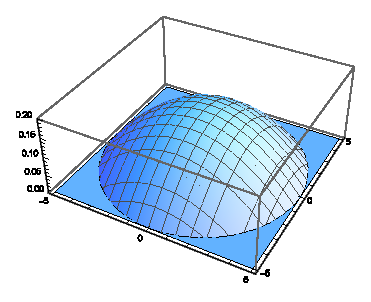
\includegraphics[width=0.5\textwidth]{3dEpanechnikov.eps}
    \caption{Epanechnikov over an area shown in 3 dimensions.}
    \label{fig:3dEpanechnikov}
\end{figure}

\Cref{fig:3dEpanechnikov} represents the distribution over a 2 dimensional space, where the third dimension represents how much the 2 dimensional points weights.

As explained earlier, the function is currently on a probability form, and not on the desired relative density form. In order to modify it, we first transform it to an absolute form. People closer to a point will weigh more than people further away from the point. We assume that every person contributes the same density, so the mean value of the function should be 1. In order to \enquote{raise} the function so the mean value is 1, we can divide by the volume beneath the plane and multiply with the desired volume. The desired volume is that of which the kernel function has a mean value of 1. We start by calculating the current volume beneath the plane. This can be done through a triple integration on the function using a circular coordinate set. As defined previously, the distance from point to center is the radius. The integration is done as shown in \cref{eq:volumeUnder3dEpanechnikov}.

\begin{equation}
\label{eq:volumeUnder3dEpanechnikov}
\int_0^{2 \pi} \int_0^h \int_0^1 \frac{3}{4 h} \left(1 - \left(\frac{r}{h}\right)^2\right) \mathrm{d}z\ \mathrm{d}r\ \mathrm{d}\theta\ = \frac{3 \pi h}{8}
\end{equation}

Because we are working in a circular coordinate system, we use three variables to index every point in the coordinate system. $z$ is the height in the circular system. $r$ is the distance from the center of the coordinate system to the point. $\theta$ is the angle in the coordinate system.

We now need to find the desired volume. Since we want a mean height to be 1, the area beneath the desired function is the same as a cylinder spanning over the same area with a height of 1. This cylinder has the area of $h^2 \cdot \pi$ where $h$ is the bandwidth. To find the absolute densities we therefore divide by the actual volume and multiply by the desired volume, as shown in \cref{eq:absoluteDensitiesEpanechnikov}.

\begin{equation}
\label{eq:absoluteDensitiesEpanechnikov}
\frac{\frac{3}{4 h} \left(1 - \left(\frac{r}{h}\right)^2\right) * \mathbbm{1}_{\{|u| \leq 1\}}}{\frac{3\pi h}{8}} * \left(h^2 \cdot \pi\right)
\end{equation}

To go from absolute densities to relative densities we simply divide by the area the absolute density has been calculated for, which is $h^2 \cdot \pi$. The relative density can then be calculated as shown in \cref{eq:relativeDensitiesEpanechnikov}.

\begin{equation}
\label{eq:relativeDensitiesEpanechnikov}
\begin{split}
&\frac{\frac{3}{4 h} \left(1 - \left(\frac{r}{h}\right)^2\right) \cdot \mathbbm{1}_{\{|u| \leq 1\}}}{\frac{3 \pi h}{8}} \cdot \frac{h^2 \cdot \pi}{h^2 \cdot \pi}\\
= &\frac{\frac{3}{4 h} \left(1 - \left(\frac{r}{h}\right)^2\right) \cdot  \mathbbm{1}_{\{|u| \leq 1\}}}{\frac{3 \pi h}{8}}\\
= &\frac{2}{\pi \cdot h^2} * \left(1-\left(\frac{r}{h}\right)^2\right) \cdot \mathbbm{1}_{\{|u| \leq 1\}}
\end{split}
\end{equation}

Finally, we simply have to sum up the relative densities for all people.

\begin{equation}
\label{eq:sumRelativeDensitiesEpanechnikov}
\frac{2}{\pi \cdot h^2} \cdot \sum_{i=1}^N \left(1-\left(\frac{d_{x,i}}{h}\right)^2 \cdot \mathbbm{1}_{\{|u| \leq 1\} }\right)
\end{equation}

Here $d_{x,i}$ is the distance from the desired point $x$ to the person $i$, and $N$ is the total amount of people. Since we have used a kernel function with a drop-off distance of h, which is the distance where all larger distances gives the value 0, in practice we only have to sum up densities for people within this radius of the point. This, as already mentioned, gives us some advantageous properties when we later in this chapter have to implement this function.

We can add some flexibility to \cref{eq:sumRelativeDensitiesEpanechnikov} by introducing an intensity variable $I$. See \cref{eq:sumRelativeDensitiesEpanechnikovWithIntensityWeight}. This variable will be utilised later in this section.

\begin{equation}
\label{eq:sumRelativeDensitiesEpanechnikovWithIntensityWeight}
\frac{2}{\pi \cdot h^2} \cdot \sum_{i=1}^N I \cdot \left(1-\left(\frac{d_{x,i}}{h}\right)^2 \cdot \mathbbm{1}_{\{|u| \leq 1\} }\right)
\end{equation}



%\includemovie[
%	poster,
%	toolbar, %same as `controls'
%	label=3depblabla.u3d,
%	text=(3depblabla.u3d),
%	3Daac=60.000000, 3Droll=0.000000, 3Dc2c=-0.000035 -3.301000 0.000000, 3Droo=3.301000, 3Dcoo=-0.000035 0.375017 0.000000,
%	3Dlights=CAD,
%]{\linewidth}{\linewidth}{figures/3depblabla.u3d}


%\pgfplotsset{width=7cm,compat=1.13}
%\usepgfplotslibrary{patchplots}
%\begin{tikzpicture}
%\begin{axis}[
%xmin=-5,xmax=5,
%ymin=-5,ymax=5,
%zmin=-0.2,zmax=0.2,
%xlabel=$x$,ylabel=$y$,ylabel=$z$]
%\addplot3[surf, patch type=rectangle, samples=40, restrict z to domain=-0.2:0] {epanechnikov3d(5)};
%addplot3[surf] {0};
%\addplot3[surf, patch type=rectangle, samples=40, restrict z to domain=0:0.2] {epanechnikov3d(5)};
%\end{axis}
%\end{tikzpicture}

\sinote*{brug det her et sted}{We assume that each person has the same density. This is done since we do not currently have a way to find the area each person takes up. This is also a reasonable assumption, and one that most crowd safety literature makes. As long as we keep the densities on 1 for the general formulas, any deviating values for the factor can simply be multiplied on the function.}
% -*- root: C:/Users/hutli/Documents/SW6/main.tex -*-

\sinote{mangler at beskrive hvordan vi bruger intensitet variablen i density og velocity, pressure og turbulens. Der mangler måske også en extension til velocity, pressure og turbulens}

\subsection{Velocity, turbulence and pressure}
This section will expand the function for kernel density estimation, found in the previous section, to functions for calculating the local crowd velocity, turbulence and pressure, the three last factors found for detecting the local crowd condition. The calculations for these crowd factors have been developed by \citet{wirz2012inferring}. The main difference between the calculations done in their paper and this project is in pressure. 

\subsubsection{Velocity}
The local crowd velocity is essentially calculated as in \citet{wirz2012inferring}. Here we use each persons velocity as the intensity of the kernel density estimation. Since we do not 

We use the relative kernel function instead of a probabilistic, as Franke et al does. Assuming that the velocity is on relative form (meters per second) both the relative and probabilistic kernel density function will give a relative local crowd velocity. This is because also divide with the kernel density sum. 
\begin{equation}
\label{eq:}
\vv{V_x} = \frac{\frac{2}{\pi \cdot h^2} \cdot \sum_{i=1}^N \vv{v_i} \cdot \left(1-\left(\frac{d_{x,i}}{h}\right)^2 \cdot \mathbbm{1}_{\{|u| \leq 1\} }\right)}{\frac{2}{\pi \cdot h^2} \cdot \sum_{i=1}^N \left(1-\left(\frac{d_{x,i}}{h}\right)^2 \cdot \mathbbm{1}_{\{|u| \leq 1\} }\right)}
\end{equation}
The function can be reduced to:
\begin{equation}
\label{eq:}
\vv{V_x} = \frac{\sum_{i=1}^N \vv{v_i} \cdot \left(1-\left(\frac{d_{x,i}}{h}\right)^2 \cdot \mathbbm{1}_{\{|u| \leq 1\} }\right)}{\sum_{i=1}^N \left(1-\left(\frac{d_{x,i}}{h}\right)^2 \cdot \mathbbm{1}_{\{|u| \leq 1\} }\right)}
\end{equation}

\subsubsection{Turbulence}

\begin{equation}
\label{eq:}
T_x = 1 - \left|\frac{\frac{2}{\pi \cdot h^2} \cdot \sum_{i=1}^{N'} h_i \cdot \left(1-\left(\frac{d_{x,i}}{h}\right)^2 \cdot \mathbbm{1}_{\{|u| \leq 1\} }\right)}{\frac{2}{\pi \cdot h^2} \cdot \sum_{i=1}^{N'} \left(1-\left(\frac{d_{x,i}}{h}\right)^2 \cdot \mathbbm{1}_{\{|u| \leq 1\} }\right)}\right|
\end{equation}

\begin{equation}
\label{eq:}
T_x = 1 - \left|\frac{\sum_{i=1}^{N'} h_i \cdot \left(1-\left(\frac{d_{x,i}}{h}\right)^2 \cdot \mathbbm{1}_{\{|u| \leq 1\} }\right)}{\sum_{i=1}^{N'} \left(1-\left(\frac{d_{x,i}}{h}\right)^2 \cdot \mathbbm{1}_{\{|u| \leq 1\} }\right)}\right|
\end{equation}

\subsubsection{Pressure}
Pressure is a bit different. The fator were originally intruduced by \citet{empircalstudy} as 
\begin{equation}
D_x \cdot \text{var}(\vv{V_x})
\end{equation}
where $D_x$ is the local crowd density and $\text{var}\vv{V_x}$ is the variance in the local crowd velocity. We use the density found in \cref{sub:kernelDensityEstimation} and multiply it with the variance introduced by Franke et al 2012 \cite{wirz2012inferring}
\begin{equation}
\label{eq:}
P_x = D_x \cdot \frac{\frac{2}{\pi \cdot h^2} \cdot \sum_{i=1}^{N} \left|\vv{v_i} - \vv{V_x}\right|^2 \cdot \left(1-\left(\frac{d_{x,i}}{h}\right)^2 \cdot \mathbbm{1}_{\{|u| \leq 1\} }\right)}{\frac{2}{\pi \cdot h^2} \cdot \sum_{i=1}^{N} \left(1-\left(\frac{d_{x,i}}{h}\right)^2 \cdot \mathbbm{1}_{\{|u| \leq 1\} }\right)}
\end{equation}
\begin{equation}
\label{eq:}
P_x = D_x \cdot \frac{\sum_{i=1}^{N} \left|\vv{v_i} - \vv{V_x}\right|^2 \cdot \left(1-\left(\frac{d_{x,i}}{h}\right)^2 \cdot \mathbbm{1}_{\{|u| \leq 1\} }\right)}{\sum_{i=1}^{N} \left(1-\left(\frac{d_{x,i}}{h}\right)^2 \cdot \mathbbm{1}_{\{|u| \leq 1\} }\right)}
\end{equation}
The main difference from this to Franke et al 2012 is that our density is relative and not probabilitylistic, meaning that the result will also be relative rather than probabilistic. \Citet{empircalstudy} did not only introduce the factor but also recorded data and pressure from an incident at \jenote{find lige ud af hvor og hvornår det uheld skete} in relative values. This means that we can in our system compare the results for specific areas with the limits and high pressure found from real world incidents, this will be used later in \jenote{referer til det sted hvor vi sætter gradienten for pres og potentiel warning layer}.
\subsection{Bandwidth Selection}

The previous parts of this section describes how we use the kernel density estimation method to calculate local crowd factors. We will now discuss the crucial part of choosing a bandwidth. We do this through a simple bandwidth selection experiment that illustrates how different bandwidths affect the results of the kernel density estimation utilised in this project.

\subsubsection{Undersmoothing and Oversmoothing}

The bandwidth is important because it controls how many data samples to include and how much they weigh. There are two extremes: a too low bandwidth or a too high bandwidth. A too low bandwidth will cause the density estimation to be noisy; the estimate will have a big variance in its output. We call this an undersmoothed estimate. The other extreme is a too high bandwidth, meaning that too many data samples would be included in the estimation, which would obscure the true density. We call this an oversmoothed estimation. An optimal bandwidth is not undersmoothed nor oversmoothed, but instead follows the structure of the true underlying density. \Cref{fig:bandwidth_selectors} explains this visually.

\begin{figure}[htbp]
\centering
    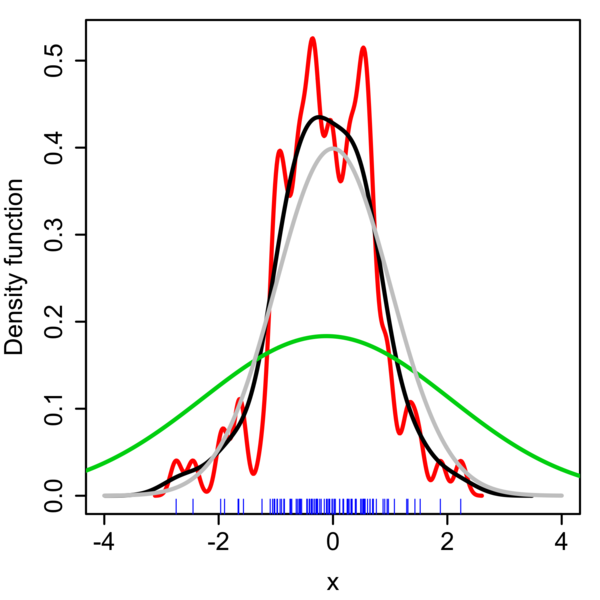
\includegraphics[width=0.5\textwidth]{bandwidth_selectors.png}
    \caption[Undersmoothing/Oversmoothing explanation]{The blue marks at the bottom of the plot shows a random sample from the Gaussian distribution. The grey curve shows the true density. The red curve visualises an undersmoothed estimation. The green curve visualises an oversmoothed estimation. The black curve is estimated using a near optimal bandwidth~\cite{wiki:kernel_density_estimation}.}
    \label{fig:bandwidth_selectors}
\end{figure}

\subsubsection{Finding a Good Bandwidth}
Finding the perfect bandwidth can be difficult. Which metrics define how good a given bandwidth is, depends on the domain of the data.

A simple approach is to eye-ball the results of using a variety of bandwidths. The result that gives the best looking bandwidth would then be chosen. This approach can give perfectly acceptable bandwidths, but the analyst has to have domain knowledge of the data. The results of this method are not reproducible, as different analysts will not deterministically choose their optimal bandwidths. Furthermore, it is also a tedious process~\cite{masteropgave}.

Another approach is to choose a bandwidth based on a metric of minimal errors. The idea is that an optimal solution will have the least errors. One method of doing this is to find the bandwidth with the lowest mean integrated squared error (MISE), as shown in \cref{eq:mise}.

\begin{equation}\label{eq:mise}
     E \int(\hat f_{h}(x) - f(x) )^2\mathrm{d}x
\end{equation}

In this method we take the integral of the squared difference between the estimate function $\hat f$ given bandwidth $h$ and the true density function $f$. We then multiply this with the expected mean value $E$ for the true density data. The intuition is that the bandwidth which will give the lowest area of error should be chosen. The hardest part of this method is to identify $f$~\cite{masteropgave}.

As noted in the introduction to this section, we will do a very simple bandwidth selection experiment. We therefore use a simpler metric of error called the sum of squared errors (SSE). The SSE is defined in \cref{eq:sse}.

\begin{equation}\label{eq:sse}
    \sum (\hat f_{h}(x) - f(x) )^2
\end{equation}

Here $\hat f_{h}(x)$ is the kernel density estimator $\hat f$ with bandwidth $h$ for a point $x$  and $f(x)$ is the actual density at point $x$. The idea of is to find the bandwidth that minimises the SSE.

The SSE formula defined in \cref{eq:sse} needs true density test data to be used as a benchmark for the performance of the bandwidth. In the perfect world, this test data should have the same structure as a real world crowd. We consider the problem of finding test data that matches a real world crowd as difficult, maybe even suitable for a project on its own. Instead, we will generate a simple pattern, that will illustrate how different bandwidths affect the kernel density estimation results.

We generate test data that takes the pattern of a chess board. This means that people has been placed such that the square alternates between two densities. The true densities are illustrated in \cref{fig:chessBoard-low1-high3-band5} where the blue squares have a density of 1 person per square metre and the turquoise squares have a density of 3 persons per square metre.

\definecolor{lowDensity}{HTML}{0967FD}
\definecolor{highDensity}{HTML}{00FFCF}

\begin{figure}[htbp]
\centering
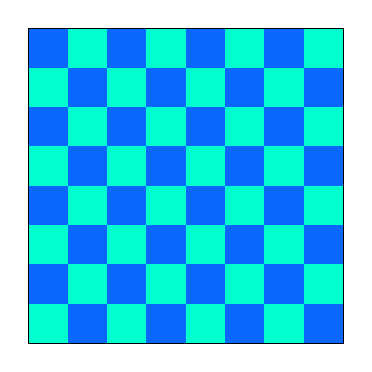
\begin{tikzpicture}[x=1cm,scale=0.5]
    \foreach \x in {0,...,7} \foreach \y in {0,...,7}
    {
        \pgfmathparse{mod(\x+\y,2) ? "lowDensity" : "highDensity"}
        \edef\colour{\pgfmathresult}
        \path[fill=\colour] (\x,\y) rectangle ++ (1,1);
    }
    \draw (0,0)--(0,8)--(8,8)--(8,0)--cycle;
\end{tikzpicture}
    \caption[Chess board pattern]{Chess board pattern with blue squares having a density of 1 person per square meter and turquoise squares having a density of 3 person per square meter.}
    \label{fig:chessBoard-low1-high3-band5}
\end{figure}

The next section will give concrete data that shows how different bandwidths affect the density estimation.

\subsubsection{Effect of Bandwidth}

Using the chess board pattern introduced in the previous section, we will now get a better intuition of the choice of bandwidth. 

\begin{figure}[htbp]
\centering

\begin{subfigure}[c]{.32\linewidth}
    \centering
    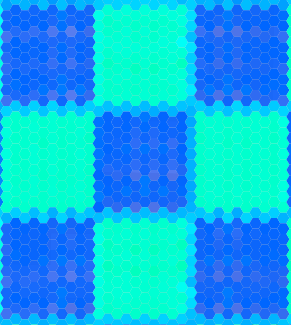
\includegraphics[width=\textwidth]{chessBoard-low1-high3-band1-density-subsquares.png}
    \caption{Bandwidth 1 metre}
    \label{fig:chessBoard-low1-high3-band1-cropped}
\end{subfigure}
%
\begin{subfigure}[c]{.32\linewidth}
    \centering
    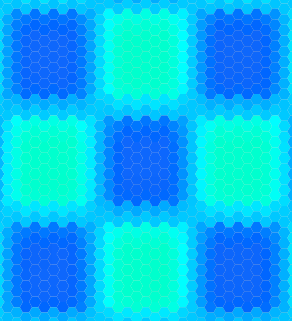
\includegraphics[width=\textwidth]{chessBoard-low1-high3-band5-density-subsquares.png}
    \caption{Bandwidth 5 metre}
    \label{fig:chessBoard-low1-high3-band5-cropped}
\end{subfigure}
%
\begin{subfigure}[c]{.32\linewidth}
    \centering
    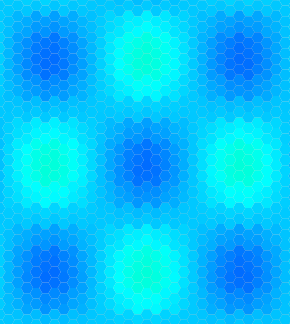
\includegraphics[width=\textwidth]{chessBoard-low1-high3-band10-density-subsquares.png}
    \caption{Bandwidth 10 metre}
    \label{fig:chessBoard-low1-high3-band10-cropped}
\end{subfigure}
%
\caption[Analysed chess board pattern with different bandwidths]{Cropped chess board pattern with blue squares having a density of 1 and turquoise squares having a density of 3. The bandwidth varies on the different subfigures.}
\label{fig:chessBoard-different-bandwidths}
\end{figure}

Let us look at how three different bandwidths change the kernel density estimation of the same data set. \Cref{fig:chessBoard-different-bandwidths} depicts three chess board patterns with varying bandwidths. \Cref{fig:chessBoard-low1-high3-band1-cropped} is very close to the structure of the chess board pattern, but there is some unwanted noise in the blue squares. We would say that the estimation is a little undersmoothed. \Cref{fig:chessBoard-low1-high3-band5-cropped} has a more blurry transition between each adjacent square, which means that the estimation is not really finding the hard transition of the underlying true data. There is however no noise inside each square. We would say that the estimation is a little oversmoothed. In \cref{fig:chessBoard-low1-high3-band10-cropped} we see a clear example of an oversmoothing bandwidth. Each square transition is still somewhat visible, but it is nowhere near the underlying true data.

Every bandwidth in \cref{fig:chessBoard-different-bandwidths} had some problems; Either the bandwidth was too low or too high. We will now try to determine a better bandwidth using the aforementioned SSE method. We iterate through a bandwidth interval from 1 metre to 5 metres with a step of 0.1 metre, because we know that the optimal bandwidth is around that interval. The result of the calculation is that the best bandwidth is 1.4 metre with an SSE of $5745.06$. \Cref{fig:chessBoard-low1-high3-band1.4-cropped} shows a crop of the chess board data with a bandwidth of 1.4 metre. We can see that this bandwidth indeed seems to be optimal; There is no noise inside the blue squares, and the square transitions are still following the underlying structure of the true density data.

\begin{figure}[htbp]
\centering
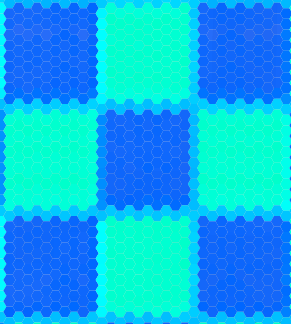
\includegraphics[width=0.32\textwidth]{chessBoard-low1-high3-band1-4-density-subsquares.png}
\caption[Analysed chess board pattern with bandwidth 1.4]{Cropped chess board pattern with blue squares having a density of 1 and turquoise squares having a density of 3. The bandwidth of 1.4 metres is calculated using a SSE method.}
\label{fig:chessBoard-low1-high3-band1.4-cropped}
\end{figure}

\subsubsection{Bandwidth Summary}

The above sample data is useful for giving an intuition of the effect of different bandwidths, but in order for the bandwidth selection to be useful in practice, one would have to do the bandwidth selection on data that represents the crowd to be analysed.


\kanote{summary af de teoretiske afsnit}